\documentclass[../calculus.tex]{subfiles}

\begin{document}

\chapter{IVT and MVT}

In this chapter we will introduce some important theorems regarding the theory of continuous and differentiable real-valued functions. Many of these are intuitive and should be familiar to the reader from learning calculus previously.

\section{Extrema and Critical Points}

One important problem in calculus is that of finding critical points and classifying (local and global) extrema that certain functions possess. It is a common scenario in applied mathematics to be faced with a function (for example, a profit function in economics) whose maximum or minimum value on its domain (i.e. global extrema) we seek the values of. There are some subtleties regarding the existence and classification of such points, and we aim to clarify such matters in this section.

\begin{definition}[Global and Local Extrema]
    \begin{shaded*}
        Let $f$ be defined on a domain $D$.
        \begin{enumerate}
            \item $f$ has an absolute (or global) maximum at $c \in D$ if $f(c) \ge f(x)$ for all $x \in D$.
            \item $f$ has a local maximum at $c$ if there exists an open interval $I$ containing $c$ such that $f(c) \ge f(x)$ for all $x \in I \cap D$.
        \end{enumerate}
        Minimums are defined analogously.
    \end{shaded*}
\end{definition}
\begin{example}
    The function $f(x)=\sin x$ on the domain $\R$ has infinitely many global minima and global maxima, occuring at values of $x$ where $f(x)=-1$ and $f(x)=1$ respectively. These values of $x$ are precisely \[x=\frac{3\pi}{2}+2n\pi\quad\text{and}\quad x=\frac{\pi}{2}+2n\pi,\quad n\in\Z,\]
    respectively.
\end{example}
One makes the natural definitions for \textit{strict} global extrema, which are unique, if they exist.

\begin{definition}[Critical Point]
    \begin{shaded*}
        A point $c$ in the domain of a differentiable function $f$ is called a critical point if either $f'(c) = 0$.
    \end{shaded*}
\end{definition}
Critical points of a differentiable function are points where the tangent line to the graph of $f$ is horizontal. However, this does \textit{not} mean that a local extremum exists there; for example, consider the function $f(x)=x^3$ on $\R$. At $x=0$, $f'(0)=0$, however the function $f$ is strictly increasing on $\R$, so $f$ admits no local or global extrema.

However, the converse is true: if a function has a local extremum at a point, and it is differentiable there, then the derivative vanishes at that point. This is called Fermat's Theorem:

\begin{theorem}[Fermat's Theorem]
    \begin{shaded*}
        Let $f$ be a function which is defined and differentiable on the open interval $(a,b)$. If $c \in (a,b)$ is a maximum (or minimum) for the function, then $f'(c) = 0$.
    \end{shaded*}
\end{theorem}
The idea is that at, say, a local maximum, the slopes from the left are positive and the slopes from the right are negative (see the picture below), and if $f$ is differentiable there, then these slopes are both converging to the same value, which must be zero by the squeeze theorem.

\begin{center}
    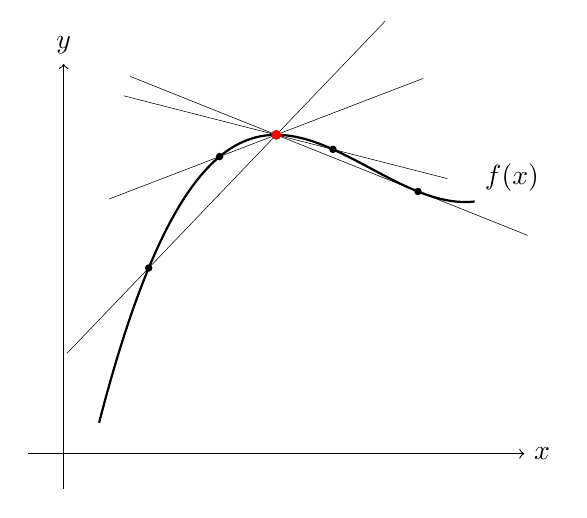
\begin{tikzpicture}[scale=0.9]

        
        \tikzset{declare function={f(\x) = 4.5 - 0.4*(\x-3)^2 + 0.1*(\x-3)^3;}}
      
        % Axes
        \draw[->] (-0.5,0) -- (6.5,0) node[right] {$x$};
        \draw[->] (0,-0.5) -- (0,5.5) node[above] {$y$};
      
        
        \draw[thick, domain=0.5:5.8, samples=150] plot (\x, {f(\x)}) node[above right] {$f(x)$};
      
       
        \coordinate (Max) at (3, {f(3)}); 
      
       
        \foreach \x in {1.2, 2.2} {
          \draw[very thin, shorten <=-1.5cm, shorten >=-2cm] (\x, {f(\x)}) -- (Max);
          \fill (\x, {f(\x)}) circle (1.5pt);
        }
      
        
        \foreach \x in {5.0, 3.8} {
          \draw[very thin, shorten <=-1.5cm, shorten >=-2cm] (\x, {f(\x)}) -- (Max);
          \fill (\x, {f(\x)}) circle (1.5pt);
        }
      
        \fill[red] (Max) circle (2pt);
      
      \end{tikzpicture}
\end{center}

\begin{example}
    Let $f(x) = x^3 - 3x$. We find the critical points by solving $f'(x) = 0$. We have $f'(x) = 3x^2 - 3 = 3(x-1)(x+1)$. Thus, $x = 1$ and $x = -1$ are critical points. Evaluating the function, $f(1) = -2$ (a local minimum) and $f(-1) = 2$ (a local maximum).
\end{example}

\section{The Mean Value Theorem}

Two results that are used to prove the Mean Value Theorem (MVT) are the Extreme Value Theorem and Rolle's Theorem (both below). Again, we prove these rigorously in Analysis I, so they will not be proved again here.

\begin{theorem}[Extreme Value Theorem]
    \begin{shaded*}
        If a function $f$ is continuous on a closed and bounded interval $[a,b]$, then $f$ attains an absolute maximum value $f(c)$ and an absolute minimum value $f(d)$ at some numbers $c, d \in [a,b]$.
    \end{shaded*}
\end{theorem}

\begin{theorem}[Rolle's Theorem]
    \begin{shaded*}
        Let $f$ be continuous on the closed interval $[a,b]$ and differentiable on the open interval $(a,b)$. If $f(a) = f(b)$, then there exists $c \in (a,b)$ such that $f'(c) = 0$.
    \end{shaded*}
\end{theorem}

\begin{theorem}[Mean Value Theorem]
    \begin{shaded*}
        Let $f$ be continuous on the closed interval $[a,b]$ and differentiable on the open interval $(a,b)$. Then there exists $c \in (a,b)$ such that
        \[f'(c) = \frac{f(b) - f(a)}{b - a}.\]
    \end{shaded*}
\end{theorem}

\begin{example}
    Consider $f(x) = x^2$ on the interval $[1, 3]$. The function is continuous on $[1,3]$ and differentiable on $(1,3)$. The average rate of change is $\frac{f(3)-f(1)}{3-1} = \frac{9-1}{2} = 4$. By the Mean Value Theorem, there exists $c \in (1,3)$ such that $f'(c) = 4$. Since $f'(x) = 2x$, solving $2c = 4$ yields $c = 2$, which lies in $(1,3)$.
\end{example}
\begin{definition}
    \begin{shaded*}
        Let $f:I\to\R$ be a function. We say that $f$ is \textit{increasing} if for all $x_1<x_2$ in $I$ we have $f(x_1)\le f(x_2)$, and \textit{decreasing} if for all $x_1<x_2$ in $I$ we have $f(x_1)\ge f(x_2)$.
    \end{shaded*}
\end{definition}
One makes the natural definitions for \textit{strictly} increasing and decreasing functions. 

A nice application of the Mean Value Theorem is the following theorem regarding the relationship between the sign of the derivative and monotonicity of differentiable functions.
\begin{theorem}[Monotonicity and Derivatives]
    \begin{shaded*}
        Let $f$ be differentiable on an interval $I$.
        \begin{enumerate}
            \item If $f'(x) > 0$ for all $x \in I$, then $f$ is strictly increasing on $I$.
            \item If $f'(x) < 0$ for all $x \in I$, then $f$ is strictly decreasing on $I$.
            \item If $f'(x) = 0$ for all $x \in I$, then $f$ is constant on $I$.
        \end{enumerate}
    \end{shaded*}
\end{theorem}
\begin{proof}
    Let $x<y$ in $I$ be arbitrary. Since $f$ is differentiable on $I$, in particular $f$ is continuous on $[x,y]$ and differentiable on $(x,y)$, so by the Mean Value Theorem there exists $c\in(x,y)$ such that \[f'(c)=\frac{f(y)-f(x)}{y-x}.\]
    Since $y-x>0$, we observe that if $f'(t)>0$ for all $t\in I$, then in particular $f'(c)>0$ so $f(y)>f(x)$, so $f$ is strictly increasing on $I$ since $x$ and $y$ were arbitrary. Similarly if $f'(t)<0$ for all $t\in I$ then $f$ is strictly decreasing on $I$. If $f'(t)=0$ for all $t\in I$ then $f(x)=f(y)$ for all $x$ and $y$ in $I$, i.e. $f$ is constant on $I$.\qedhere 
\end{proof}

\begin{example}
    We will prove the inequality $\sin x\le x$ for $x\ge 0$. Define $g:[0,\infty)\to\R$ by $g(x)=x-\sin x$; then $g(0)=0$ and $g$ is differentiable with \[g'(x)=1-\cos x\]for all $x\ge 0$. Since $|\cos x|\le 1$ for all $x\in\R$, we have $g'(x)\ge 0$ for all $x\ge 0$, so the function $g$ is increasing on $[0,\infty)$, so since $g(0)=0$, $g(x)\ge 0$ for all $x\ge 0$, i.e. $\sin x\le x$ for all $x\ge 0$, as required.
\end{example}

\section{Intermediate Value Theorem}

A very intuitive theorem, but one that is not so easy to prove (again, we prove this theorem rigorously in Analysis I) is the Intermediate Value Theorem (IVT), which intuitively states that continuous functions cannot ``jump'' over values.

\begin{theorem}[Intermediate Value Theorem]
    \begin{shaded*}
        Let $f$ be a continuous function on the closed interval $[a,b]$. If $y$ is any number strictly between $f(a)$ and $f(b)$, then there exists $c \in (a,b)$ such that $f(c) = y$.
    \end{shaded*}
\end{theorem}
Practically, one example where this theorem is useful is for estimating when roots of continuous functions exist.

\begin{example}
    We show that the equation $x^3 - x - 1 = 0$ has a root in the interval $[1,2]$. Let $f(x) = x^3 - x - 1$. Since $f$ is a polynomial, it is continuous everywhere. We evaluate the endpoints: $f(1) = 1 - 1 - 1 = -1$ and $f(2) = 8 - 2 - 1 = 5$. Since $f(1) < 0 < f(2)$, the Intermediate Value Theorem guarantees the existence of a $c \in (1,2)$ such that $f(c) = 0$.
\end{example}



\end{document}